\apendice{Documentación técnica de programación}

\section{Introducción}

El objetivo de este Apéndice es documentar a nivel técnico el presente proyecto, con objetivo de permitir la instalación en local del proyecto, facilitar el acceso a  un entorno de desarrollo y la extensión del proyecto.

\section{Estructura de directorios}

Todo el proyecto se ha desarrollando utilizando en un único repositorio \texttt{git} para control de versiones, que está disponible en el siguiente enlace: \url{https://github.com/dpuertamartos/big_data_tfm}.

Dentro del directorio raíz del repositorio, encontramos las carpetas mostradas en la Figura \ref{fig:dirtree_general} y además algunos archivos fundamentales para el proyecto. 

En la mayoría de las carpetas del repositorio, excepto \texttt{Latex}, \texttt{airflow} y \texttt{utils}, encontraremos un archivo con nombre \textit{Dockerfile}, que es el archivo de configuración del contenedor de Docker (Ver Sección \ref{sec:implementacion_docker}). En el servicio Airflow no es necesario dicho archivo, pues se usa una imagen oficial. En la carpeta \texttt{utils} simplemente se encuentra un \textit{script} que se corre periódicamente para renovar el certificado https, no siendo estrictamente necesario para el funcionamiento del proyecto.


\begin{figure}
	\dirtree{%
		.1 /big\_data\_tfm/ . 
            .2 Latex \textit{(Memoria del Proyecto)}.
            .3 img.
            .3 tex.
		.2 ETL \textit{(Servicio de ETL) \ref{sec:etl_section}}. 
            .2 ingestion\_scrapper \textit{(Servicio de scraping) \ref{sec:scrapy_section}}.
            .3 ingestion\_scrapper.
            .4 spiders.
            .4 fixes.
            .2 data\_analysis \textit{(Servicio de Aprendizaje Automático) \ref{sec:ml_section}}.
            .2 airflow \textit{(DAGs de Airflow) \ref{sec:airflow_section}}. 
            .3 dags.
            .2 backend \textit{(Backend del sitio web) \ref{sec:backend_section}}.
            .3 controllers.
            .3 requests.
            .3 util.
            .2 frontend \textit{(Frontend del sitio web) \ref{sec:frontend_section}}.
            .3 public.
            .3 src.
            .2 utils.
            .2 README.md \textit{(Documentación resumida)}.
            .2 architecture.drawio \textit{(Esquema de arquitectura)}.
            .2 docker-compose.yaml \textit{(Configuración de Docker Compose)}.
	}
	\caption{Árbol de directorios General}
	\label{fig:dirtree_general}
\end{figure}

\clearpage
\section{Manual del programador}

En esta sección se entrará más en detalle en como está estructurado y configurado el código, habrá una subsección para cada servicio (titulada con el nombre de la carpeta en el repositorio que aloja el código de dicho servicio) y una para las bases de datos.

Algunos aspectos generales que se mencionaran previamente para no repetirlos en cada subsección son los siguientes:

\begin{itemize}
    \item \texttt{requirements.txt}: Se tratan de archivos que describen las dependencias del servicio. Generados mediante el comando \texttt{pip freeze > requirements.txt}. Posteriormente se usan en el flujo de Docker para instalar dependencias. Usado para servicios que usan Python.
    \item \texttt{package.json}: Archivos de dependencias para los servicios web, gestionados por \texttt{npm}. Usado para servicios que usan Javascript (web).
    \item \texttt{Dockerfile}: Archivo de configuración de la imagen de Docker.
    \item \texttt{readme.md}: Archivos con documentación del servicio.
    \item Scripts shell (\texttt{.sh}): Actúan como vínculo entre el orquestador (Apache Airflow) y el propio servicio. Generalmente lanzan archivos \texttt{.py} y guardan \textit{logs}. Son ejecutados por el contenedor de Docker cuando este se lanza a través de Airflow.
\end{itemize}

\clearpage
\subsection{ingestion\_scrapper - Servicio de Scrapy}

Este servicio está escrito completamente en Python y sigue el esquema a creado tras ejecutar el comando \texttt{scrapy startproject ingestion\_scrapper}. En este proyecto los ficheros añadidos, modificados e inalterados respecto a la plantilla generada tras iniciar el proyecto, se muestran en la Figura \ref{fig:dirtree_scrapy}. Este servicio está pensado para funcionar con ejecuciones individualizadas, así, cada vez se lanza un contenedor de Docker que posteriormente se elimina. Con dicho contenedor, se puede lanzar tanto el servicio de recogida de datos de inmuebles (actualmente, 2 veces al día), como el servicio de comprobación de si los anuncios siguen activos (actualmente, 1 vez al día), según el \textit{Script} de Shell que lance.

Algunos detalles que merece la pena mencionar con los siguientes:

\begin{itemize}
    \item Carpeta \texttt{.../fixes/}: En esta carpeta se han recogido algunos scripts que se fueron utilizando a lo largo de los meses para adaptar el proyecto a nuevas funcionalidades. A día de hoy son prescindibles y no son necesarios para el funcionamiento del proyecto. Por ejemplo, encontramos un script \texttt{script\_to\_add\_active\_field.py}, que se usó para añadir el campo \texttt{active} a todos los inmuebles en la distintas colecciones de la MongoDB.
    \item Archivo \texttt{settings.py}: Desde aquí se modifica el comportamiento general de Scrapy
    \item Carpeta \texttt{.../spiders/}: Esta es la carpeta que realmente personaliza la funcionalidad del servicio de \textit{Scraping}. 
    
    Encontramos dos ``arañas'' distintas: una llamada \texttt{/spiders/pisos\_spider.py}, que es la que contiene toda la lógica para recopilar la información de inmuebles y otra,  \texttt{/spiders/check\_up\_spider.py}, que es la que contiene toda la lógica de verificar sin un anuncio sigue disponible o no.
    \item Los scripts de shell: \texttt{ingestion\_script.sh}, \texttt{ad\_up\_checking\_script.sh}. Son el punto único de enlace entre el orquestador y los dos tipos de tarea: La de recopilación/ingestión de inmuebles y la de comprobar si un anuncio sigue activo. Estos scripts generan logs que se almacenan en un volumen de Docker.
\end{itemize}


\begin{figure}
	\dirtree{%
		.1 /big\_data\_tfm/.
            .2 /ingestion\_scrapper/.
            .3 requirements.txt.
            .3 Dockerfile.
            .3 scrapy.cfg \textit{(Original)}.
            .3 /ingestion\_scrapper/.
            .4 /fixes/.
            .5 script...py \textit{(Scripts de uso único)}.
            .4 /spiders/.
            .5 \_\_init\_\_.py .
            .5 pisos\_spider.py \textit{(Añadido)}.
            .5 check\_up\_spider.py \textit{(Añadido)}.
            .4 \_\_init\_\_.py.
            .4 items.py \textit{(Original)}.
            .4 middlewares.py \textit{(Original)}.
            .4 pipelines.py \textit{(Original)}.
            .4 settings.py \textit{(Modificado)}.
            .4 config.py \textit{(Añadido)}.
            .4 ingestion\_script.sh \textit{(Añadido)}.
            .4 ad\_up\_checking\_script.sh \textit{(Añadido)}.
	}
	\caption{Árbol de directorios de servicio \textit{Scrapy}}
	\label{fig:dirtree_scrapy}
\end{figure}

\clearpage
\subsection{ETL}

Este servicio también está escrito completamente en Python, usando principalmente la librería Pandas~\cite{pandas}. Este servicio engloba dos tareas de las orquestadas por Airflow:

\begin{itemize}
    \item Transformación (ETL en sí): Lee de las colecciones de MongoDB y da lugar a la tabla \texttt{pisos} en SQLite (Ver subsección \ref{subsec:tabla_pisos}).
    \item Agregación: Lee de la tabla \texttt{pisos} y genera la tabla \texttt{pisos\_dw} (Ver subsección \ref{subsec:tabla_pisos}).
\end{itemize}

De igual forma que el servicio de \textit{Scrapy}, este servicio está pensado para funcionar con ejecuciones individualizadas, lanzando un contenedor de Docker que realizará una función según el \textit{Script} de Shell que lance. En la actualidad se ejecuta el servicio de transformación dos veces al día, seguido del de agregación. Se detallan los archivos en Figura \ref{fig:dirtree_ETL}.


\begin{figure}
	\dirtree{%
		.1 /big\_data\_tfm/.
            .2 /ETL/.
            .3 requirements.txt.
            .3 Dockerfile.
            .3 config.py.
            .3 aggregation.py \textit{(Principal Agregación)}.
            .3 extraction.py \textit{(ETL)}.
            .3 transformation.py \textit{(ETL)}.
            .3 transformation\_utils.py \textit{(ETL)}.
            .3 loading.py \textit{(ETL)}.
            .3 main.py \textit{(Principal ETL)}.
            .3 transformation\_script.sh \textit{(ETL)}.
            .3 aggregation\_script.sh \textit{(Agregación)}.
        }
	\caption{Árbol de directorios de servicio de ETL y Agregación}
	\label{fig:dirtree_ETL}
\end{figure}

\clearpage
\subsection{data\_analysis - Servicio de Aprendizaje Automático}

Este servicio se basa en el paquete \texttt{scikit learn}~\cite{scikit-learn} y está escrito en Python. Por una parte consta del código que entrena y genera los modelos, cuyo archivo principal es \texttt{train.py}, este utiliza funciones de \texttt{model\_generation.py}, y crea y almacena un ``limpiador/transformador'' final de los datos utilizando \texttt{data\_cleaning.py}. Este flujo de entrenamiento acaba con el almacenamiento permanente de los modelos y el ``limpiador'' en un volumen de Docker.

En el flujo de predicción, mucho más simple, encontramos solamente \texttt{generate\_predictions.py}. Este flujo carga los modelos y el limpiador de datos para aplicarlos las entradas más recientes de la tabla \texttt{pisos}.

Los datos se leen directamente de la tabla \texttt{pisos} de SQLite tanto para el entrenamiento (en este caso se leen datos de como máximo 6 meses de tiempo), como para el flujo de predicción de valor/puntuación, en este caso se leen los datos que aún no tienen predicción asignada.

Como entrada al código de Python, para cada uno de los dos flujos, encontramos de nuevo dos \textit{Scripts} de Shell: \texttt{predict.sh} y \texttt{train.sh}. Como pasaba para el servicio de \textit{Scrapy} y ETL, este servicio funciona con la construcción de un contenedor de Docker temporal, que llama a uno de estos dos \textit{Scripts} según la tarea y es orquestado por Airflow.

\begin{figure}
	\dirtree{%
		.1 /big\_data\_tfm/.
            .2 /data\_analysis/.
            .3 requirements.txt.
            .3 Dockerfile.
            .3 config.py.
            .3 convert\_db\_to\_csv.py
            .3 data\_cleaning.py.
            .3 model\_generation.py.
            .3 train.py.
            .3 generate\_predictions.py.
            .3 predict.sh \textit{(Regresión de Precio)}.
            .3 train.sh \textit{(Entrenamiento de modelos)}.
        }
	\caption{Árbol de directorios de servicio de Aprendizaje Automático}
	\label{fig:dirtree_ml}
\end{figure}

\clearpage
\subsection{airflow - Servicio de Airflow}

El servicio de Airflow se basa en la imagen \texttt{apache/airflow:2.7.1}. Así, se despliegan dos contenedores permanentes (a diferencia de los servicios anteriores), uno para \textit{webserver} (interfaz web de Airflow) y otro para \textit{scheduler}, para ver más detalles se puede ver el archivo \texttt{docker-compose.yaml} del proyecto.

Para iniciar correctamente el servicio por primera vez hay que seguir las instrucciones explicadas en Sección \ref{sec:instalacion_despliegue}.

Una vez en funcionamiento los contenedores y seguidas las instrucciones de instalación, los únicos archivos que encontramos en el proyecto son los relacionados con las DAGs~\cite{dags}, es decir los que indican las tareas a orquestar por Airflow, almacenados en \texttt{/big\_data\_tfm/airflow/dags/}. Estos archivos que configuran las DAGs se montan en los contenedores de Airflow.

Debemos tener en cuenta que todas las tareas de Airflow consisten en desplegar un contenedor de Docker temporal. Las podemos ver en Tabla \ref{table:dags}. Para más detalle se recomienda consultar el código de dichas DAGs.

\begin{table}[H]
\centering
\begin{tabular}{|l|l|l|}
\hline
\textbf{DAG} & \textbf{Frecuencia} & \textbf{Tareas} \\
\hline
\texttt{ingestion\_and\_ETL\_dag} & 2 por día & 
\texttt{ingestion\_task} \\
.py & & \texttt{checking\_deletes\_task} \textit{(1/día)} \\
& & \texttt{transformation\_task} \\
& & \texttt{aggregation\_task} \\
& & \texttt{prediction\_task} \\
\hline
\texttt{train\_dag.py} & 1 por mes & \texttt{training\_task} \\
& & \texttt{prediction\_task} \\
\hline
\texttt{mongo\_backup\_dag.py} & Cada 3 días & \texttt{mongo\_backup\_task} \\
\hline
\texttt{initial\_run\_dag.py} & Solo manual& Regenera el proyecto. \\
& & Utiliza una MongoDB restaurada \\
\hline
\end{tabular}
\caption{Descripción de las DAGs en Apache Airflow}
\label{table:dags}
\end{table}

\clearpage
\subsection{backend - Servicio \textit{Backend} de la Web}

Este servicio se compone de un servidor Node.js utilizando el framework Express, desarrollado completamente en JavaScript. El objetivo principal de este servicio es facilitar la comunicación entre la base de datos SQLite y la interfaz de usuario (\textit{Frontend}) del sitio web.

\paragraph{Arquitectura y Componentes Clave: } La arquitectura del servicio de backend está diseñada para ser modular, permitiendo una fácil expansión y mantenimiento (Ver Figura \ref{fig:dirtree_backend}). Los componentes clave incluyen:

\begin{itemize}
    \item \textbf{Controllers}: Carpeta \texttt{/controllers} contiene archivos como \texttt{flats.js} y \texttt{trends.js}, que definen las rutas de la API y los controladores asociados a ellas. Estos controladores procesan las peticiones entrantes, interactúan con la base de datos y devuelven las respuestas adecuadas al cliente.
    \item \textbf{Utilidades}: La carpeta \texttt{/util} incluye archivos cruciales como \texttt{config.js} para la configuración del entorno, \texttt{db.js} que maneja la conexión y operaciones de la base de datos, \texttt{logger.js} para el registro de actividades y errores, utilizado por middleware
    \texttt{middleware.js} que contiene middleware para manejo de errores, y \textit{logging}.
    \item \textbf{Configuración y Despliegue}: Archivos como \texttt{.dockerignore}, \texttt{.eslintrc.js}, y \texttt{.gitignore} configuran aspectos del entorno de desarrollo, \textit{linting} y versionado, respectivamente. \texttt{Dockerfile} permite la contenerización del servicio para un despliegue eficiente y consistente. 
    \item \textbf{Punto de Entrada}: \texttt{app.js} configura la aplicación Express, estableciendo middlewares y rutas principales, mientras que \texttt{index.js} sirve como el punto de entrada del servicio, iniciando el servidor y realizando configuraciones iniciales.
    \item \textbf{Gestión de Dependencias}: \texttt{package.json} y \texttt{package-lock.json} gestionan las dependencias del proyecto, asegurando versiones consistentes de las librerías y facilitando la instalación y actualización de paquetes.
\end{itemize}

\paragraph{Funcionamiento y Flujo de datos: }
Cuando una solicitud es recibida por el servidor, es procesada por el middleware correspondiente. Después, la solicitud es dirigida al controlador adecuado, donde se realizan operaciones específicas, como consultas o actualizaciones en la base de datos, antes de enviar una respuesta al cliente.

\begin{figure}
    \dirtree{%
        .1 /big\_data\_tfm/.
            .2 /backend/.
                .3 /controllers/.
                    .4 flats.js.
                    .4 trends.js.
                .3 /util/.
                    .4 config.js.
                    .4 db.js.
                    .4 logger.js.
                    .4 middleware.js.
                .3 .dockerignore.
                .3 .eslintrc.js.
                .3 .gitignore.
                .3 Dockerfile.
                .3 app.js.
                .3 index.js.
                .3 package.json.
                .3 package-lock.json.
    }
    \caption{Árbol de directorios del \textit{Backend} de la web}
    \label{fig:dirtree_backend}
\end{figure}


\subsection{frontend - Servicio \textit{Frontend} de la Web}

El servicio \textit{Frontend} está desarrollado utilizando React, una librería de JavaScript para construir interfaces web para el usuario. Se comunica con el servicio de \textit{Backend} para obtener y enviar datos, lo que permite a los usuarios interactuar con la información almacenada en la base de datos de forma intuitiva. La estructura del proyecto \textit{Frontend} se organiza según lo mostrado en la Figura \ref{fig:dirtree_frontend}.

En la carpeta \texttt{/public/} encontraremos recursos estáticos, imágenes e iconos que se usan en la aplicación. Dentro de la carpeta \texttt{/src/}, encontraremos las siguientes subcarpetas y archivos importantes:

\begin{itemize}
    \item \texttt{/assets/}: Contiene otros recursos estáticos
    \item \texttt{/components/}: Aquí se almacenan los componentes React, que son las unidades básicas de construcción de la interfaz de usuario. Cada componente (\texttt{.jsx}) representa una parte de la interfaz, como la página de inicio, la lista de pisos, las tendencias, el contacto y el pie de página. A su vez estas páginas están divididas en otros componentes
    \item \texttt{/services/}: Incluye servicios para la comunicación con el backend, como la obtención de datos de pisos y tendencias
    \item \texttt{/utils/}: Ofrece utilidades y funciones auxiliares, como opciones de selectores que son usadas a través de la aplicación
    \item \texttt{App.jsx}: El componente principal que engloba toda la aplicación React. En él se define la barra de navegación
    \item \texttt{index.css}: Hoja de estilos principal para la aplicación. No se ha utilizado demasiado, ya que se ha optado por dar la mayoría de los estilos dentro de los componentes.
    \item \texttt{main.jsx}: Punto de entrada de la aplicación React, donde se monta el componente principal \texttt{App}
\end{itemize}

Fuera de las carpetas \texttt{/public/} y \texttt{/src/}, encontramos varios archivos y configuraciones relevantes para el proyecto:

\begin{itemize}
    \item \texttt{.dockerignore}, \texttt{.eslintrc.js}, \texttt{.gitignore}: Archivos de configuración para Docker, ESLint y Git, respectivamente, que ayudan a gestionar el entorno de desarrollo y control de versiones.
    \item \texttt{Dockerfile}: Define las instrucciones para crear una imagen Docker del servicio 
    \item \texttt{package.json} y \texttt{package-lock.json}: Estos archivos gestionan las dependencias del proyecto, especificando las librerías y paquetes necesarios para el desarrollo y ejecución de la aplicación.
    \item \texttt{vite.config.js}: Configuración de Vite~\cite{vite} específica para este proyecto, optimizando el proceso de construcción y desarrollo.
    \texttt{provinces.json}: Un archivo de datos utilizado por la aplicación, datos estáticos.
\end{itemize}

Utilizando Vite~\cite{vite}, un paquete para crear rápidamente plantillas para aplicaciones React, este proyecto \textit{Frontend} aprovecha una compilación rápida y un servidor de desarrollo eficiente con autorecarga cuando se cambia algún componente, lo que resulta en una mejora significativa en la velocidad de desarrollo.

\begin{figure}
    \dirtree{%
        .1 /big\_data\_tfm/.
            .2 /frontend/.
                .3 /public/.
                    .4 flats.jpg.
                    .4 favicon.ico.
                .3 /src/.
                    .4 /assets/.
                        .5 react.svg.
                    .4 /components/.
                        .5 Home.jsx.
                        .5 Flats.jsx.
                        .5 Trends.jsx.
                        .5 Contact.jsx.
                        .5 Footer.jsx.
                        .5 ....jsx.
                    .4 /services/.
                        .5 flats.js.
                        .5 trends.js.
                    .4 /utils/.
                        .5 selector\_options.js.
                    .4 App.jsx.
                    .4 index.css.
                    .4 main.jsx.
                .3 .dockerignore.
                .3 .eslintrc.js.
                .3 .gitignore.
                .3 Dockerfile.
                .3 index.html.
                .3 index.js.
                .3 package.json.
                .3 package-lock.json.
                .3 vite.config.js.
                .3 README.md.
                .3 provinces.json.
                }
    \caption{Árbol de directorios del \textit{Frontend} de la web}
    \label{fig:dirtree_frontend}
\end{figure}

\clearpage
\subsection{Bases de datos: MongoDB y SQLite}

\paragraph{La base de datos MongoDB: }Su elección y utilidad se explica en la Sección \ref{sec:mongodb_section}, funciona con un contenedor de Docker que utiliza la última imagen disponible \texttt{mongo:latest}, y almacena los datos en un volumen (\texttt{mongodb-data}) montado en el contenedor. No necesita ningún tipo de instalación más que seguir el procedimiento de la Sección \ref{sec:instalacion_despliegue}

En el archivo \texttt{/big\_data\_tfm/readme.md}, existe una sección titulada \texttt{6. MongoDB} donde se explica como restaurar un \textit{backup} de mongodb. Estos \textit{backups} se generan cada 3 días si se activa el DAG \texttt{mongo\_backup\_dag.py} (Ver Tabla \ref{table:dags}). Para mover dicho \textit{backup} del volumen \texttt{\{project\}\_mongodb-backups} al sistema de archivos local se puede seguir la sección titulada \texttt{8. DEV-UTILS} del archivo \texttt{readme.md.}

Esta base de datos es la clave del proyecto, y utilizando un \textit{backup} de la misma, se puede regenerar la base de datos SQLite, los modelos y continuar con el proceso de \textit{scraping} desde un punto anterior, aunque hayan pasado múltiples días/semanas e incluso meses sin actualización.

\paragraph{La base de datos SQLite: } Se trata únicamente de un archivo nombrado \texttt{pisos.db}, que se genera por primera vez, si no existe, tras ejecutar la tarea de ETL. Este archivo se almacena en un volumen de Docker que se monta en los distintos contenedores (Ver archivo \texttt{docker-compose.yaml} y observar volumen nombrado como \texttt{sqlite-db}).

Es extremadamente sustituible, esta base de datos completa se puede regenerar en pocos minutos a partir de una copia de la base de datos MongoDB, por ello no se realizan \textit{backups}. Su mayor utilizad es dar rápido acceso a datos estructurados/tabulares por la web y los tareas de Aprendizaje Automático.

\clearpage
\section{Compilación, instalación y ejecución del proyecto}\label{sec:instalacion_despliegue}

En esta sección se abordará como ejecutar el proyecto completo en un entorno local. Aunque el proyecto está desplegado en una máquina virtual de Oracle Cloud, podría ser desplegado en cualquier máquina de forma similar, incluida la web.

Solo se abordará la ejecución mediante Docker, ya que es la única solución unificada. Sin embargo, sería totalmente posible la instalación y ejecución de cada uno de los servicios sin utilizar ningún tipo de contenedor, aunque no está explicada ni soportada en esta memoria por su extensión. Cabe señalar que hay mucha información ampliada en el archivo \texttt{/big\_data\_tfm/readme.md}, disponible para consulta si se quieren más detalles.

Los prerequisitos son los siguientes:

\begin{itemize}
    \item Docker instalado
    \item Terminal Unix (Compatible WSL de Windows)
    \item Dar permisos de escritura y lectura en el socket de Docker para todos los usuarios. Esto es necesario para que Airflow utilice el socket. 
    
    \texttt{sudo chmod 666 /var/run/docker.sock}
    
\end{itemize}

A continuación necesitamos completar algunos pasos imprescindibles, antes de tener el proyecto en funcionamiento:

\begin{itemize}
    \item Clonar repositorio

    \texttt{git clone https://github.com/dpuertamartos/big\_data\_tfm.git}

    \item Iniciar la base de datos de Airflow

    \texttt{docker-compose run --rm airflow\_webserver airflow db init}

    \item Crear usuario para Airflow. Por defecto, usuario \texttt{admin}, password \texttt{admin}.

\begin{lstlisting}
docker-compose run \
--rm airflow_webserver airflow \
users create \
--username admin \
--firstname FIRST_NAME \
--lastname LAST_NAME \
--role Admin \
--email admin@example.org \
--password admin 
\end{lstlisting}

    \item Construir contenedores para \textit{Scraping}, ETL y Aprendizaje Automático. Estos contenedores son lanzados y destruidos tras cada ejecución, no están continuamente activos.

    \texttt{docker-compose build scraper etl data\_analysis}

    \item Lanzar contenedores para Airflow, Mongodb y la web

    \texttt{docker-compose up -d mongodb airflow\_webserver airflow\_scheduler app backend nginx}

    Se debe tener en cuenta que la web en local no mostrará datos hasta que pasen unos días con el servicio de ingestión o bien se regeneren las bases de datos a partir de un \textit{backup} (Explicado en subsección \ref{sec:regenerar_desde_backup}).

    \item Acceder a interfaz de Airflow en el Navegador \texttt{http://0.0.0.0:8080/}:
    
    Como mínimo se debe activar la DAG \texttt{ingestion\_transformation\_dag}, que iniciará la recogida de datos. 
    
    Se recomienda activar \texttt{training\_dag}, solo si ya se tienen unas semanas de recogida de datos o si se ha partido de un \textit{backup} de MongoDB y se ha lanzado ya \texttt{initial\_run\_dag}.

    Opcionalmente podemos activar \texttt{mongo\_backup\_dag} si queremos que se realice un backup del volumen que contiene los datos de MongoDB cada tres días.

    En la Figura \ref{fig:airflow_interfaz} se pueden ver las DAGs activadas en una ejecución del producto madurada durante varios meses. 
\end{itemize}

\begin{figure}[ht]
    \centering
	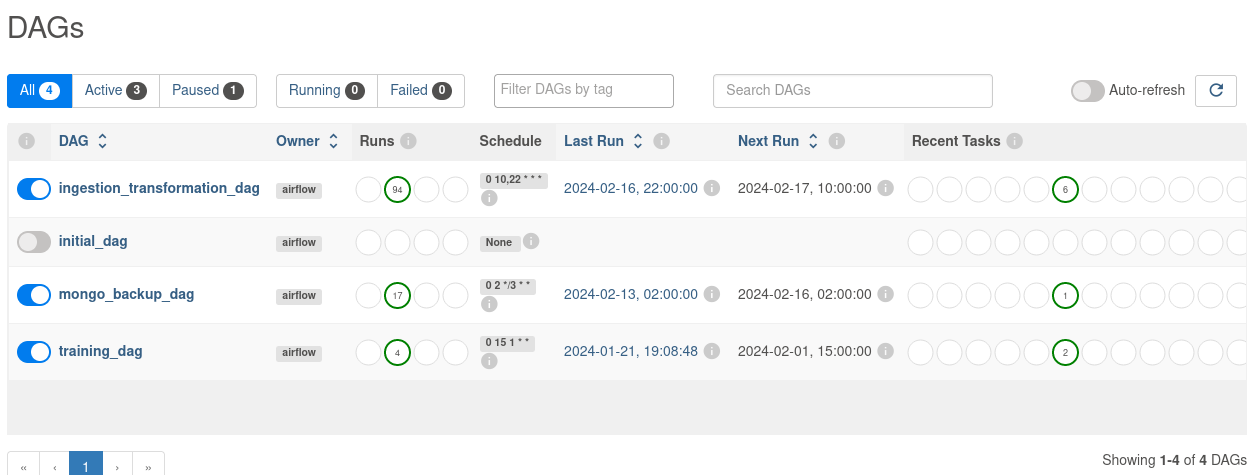
\includegraphics[width=1\textwidth]{img/airflow_interfaz.PNG}
	\caption[Interfaz de Apache Airflow Web Server, con DAGs del proyecto]{Interfaz de Apache Airflow Web Server, con DAGs del proyecto activadas en la máquina del entorno de producción. Se activan pulsando el \textit{slider} azul/gris a la izquierda del nombre.}
	\label{fig:airflow_interfaz}
\end{figure}

\clearpage
\section{Cómo regenerar todo el proyecto desde un \textit{backup} de MongoDB}\label{sec:regenerar_desde_backup}

Primero, debemos restaurar los datos en MongoDB, el proceso de recuperación dependerá de como se ha generado el \textit{backup}. Si se trata de un \textit{backup} generada a través de la DAG de este proyecto destinada a tal causa, seguiremos los siguientes pasos después de clonar el repositorio (Se deben cumplir los prerrequisitos de la Sección \ref{sec:instalacion_despliegue}):

\begin{itemize}

    \item Si existe un volumen previo con datos de MongoDB, lo borramos

    \texttt{docker volume remove big\_data\_tfm\_mongodb-data}
    
    \item Iniciamos el contenedor de MongoDB, creando el volumen de datos asociado:
    
    \texttt{docker compose up -d mongo}
    
    \item Descomprimiremos el \textit{backup} obteniendo una carpeta denominada \textit{mongo\_backup} o similar

    \item Copiaremos el \textit{backup} dentro de una carpeta temporal del contenedor

    \texttt{docker cp /path/to/backup/mongo\_backup/ mongodb-container:/tmp/bkup}

    \item Restauraremos el \textit{backup} con el siguiente comando

    \texttt{docker exec -it mongodb-container mongorestore /tmp/bkup}

    \item Eliminamos la carpeta temporal del contenedor

    \texttt{docker exec mongodb-container rm -rf /tmp/bkup}
    
    
\end{itemize}

Posteriormente continuaremos con los pasos de la sección \ref{sec:instalacion_despliegue} y al llegar al apartado de iniciar las DAGs, deberemos activar manualmente la DAG \texttt{initial\_run\_dag} una sola vez, esto regenerará la base de datos SQLite y se entrenaran los modelos (Puede tardar un par de horas según la máquina). Finalmente, tras el éxito de regenerar el resto de elementos a partir del \textit{backup} de MongoDB, ya podemos activar las DAGs como aparece en la Figura \ref{fig:airflow_interfaz}, tendremos todos los servicios orquestados y la web disponible con los datos hasta el punto que tuviese almacenado el \textit{backup}.
